\section{Experiments}
\label{sec:exp}
\subsection{Experimental setup}
\paragraph{Real LLM and benchmark.}
\emph{Data.} MMLU-Pro \citep{wang2024mmlupro} (dataset revision \texttt{b189ec7}, 12\,032 test questions, up to 10 options). We fix a uniformly random population $P$ of $\RealN$ test questions; the remaining questions are never used. The 70 validation questions provide few-shot demonstrations.
\emph{Model.} Qwen2.5-1.5B-Instruct \citep{qwen2024qwen25}, 8-bit GGUF, run with llama.cpp on CPU; the answer is the option letter with the largest next-token log-probability (greedy, deterministic, no chain of thought), so a (configuration, question) pair has one fixed outcome.
\emph{Configuration space} ($K{=}72$): option format (\texttt{A.\ text} / \texttt{(A) text}) $\times$ demonstrations (none / one of two fixed 3-shot sets) $\times$ one of 4 instruction sentences $\times$ one of 3 answer cues. This is a small, hand-built space of the kind that instruction/demonstration optimisers explore, evaluated exhaustively so that every search is a replay on a complete per-item score matrix $Y\in\{0,1\}^{|P|\times 72}$.
\emph{Benchmark draws and truth.} Each replicate draws a benchmark $S$ of $n\in\{50,100,200,400,800\}$ questions i.i.d.\ (with replacement) from $P$, and the true performance of a configuration is its exact accuracy over $P$: the empirical distribution of $P$ plays the role of the task distribution. (Drawing $S$ without replacement and scoring on $P\setminus S$ is also possible, but then the fresh accuracy is mechanically anti-correlated with the benchmark accuracy and the measured optimism is inflated by $|P|/(|P|-n)$; App.~\ref{app:wr} reports this secondary design for small $n$.) \emph{Search procedures} (each sees only $S$): random search with budget $B\in\{1,\dots,72\}$ and full evaluation of each candidate; successive halving (3-way, nested subsets of $S$, final rung on all of $S$); greedy coordinate ascent over the three factors from a random start; and a surrogate-guided search in the style of MIPRO \citep{opsahl2024optimizing}: 40 trials on random minibatches of 50 questions proposed from an additive per-factor surrogate, then full evaluation of the 3 best. These are our own implementations of the algorithm families, \emph{not} the DSPy code (Sec.~\ref{sec:disc}).

\paragraph{Synthetic worlds.}
To control the quantities that theory says matter and to reach regimes the real pool does not contain, we simulate item-level outcomes from a latent-threshold model with the same factorial configuration structure: $y_{ci}=\mathbb 1[a+\mu_c+\sqrt{\rho}\,z_i+\sqrt{1-\rho}\,u_{ci}>0]$, $z_i,u_{ci}\sim\mathcal N(0,1)$, where $\mu_c$ (standardised to SD $\tau$) mixes additive factor effects and interactions, $\rho$ is the latent between-configuration correlation (item difficulty shared by all configurations), and $a$ sets base accuracy. We also use i.i.d.\ configuration effects with normal, sparse (5\% of configurations much better), heavy-tailed ($t_3$) and bimodal (half the configurations ``broken'') distributions for robustness checks.

\paragraph{Metrics.}
For each reporting method: \emph{bias} $=\mathbb{E}[\text{report}-\mu(\hat\theta)]$, \emph{RMSE}, \emph{coverage} and median width of nominal-95\% intervals for $\mu(\hat\theta)$ (the quality of the configuration that would actually be deployed), and, for comparisons, the rate of significant ``$A>B$'' claims at one-sided level 5\% against the true gap. Monte-Carlo errors are reported (bias: $\pm1.96$ SE; coverage: binomial SE).


\subsection{How large is the gap, and what drives it?}
\begin{figure}[t]
\centering
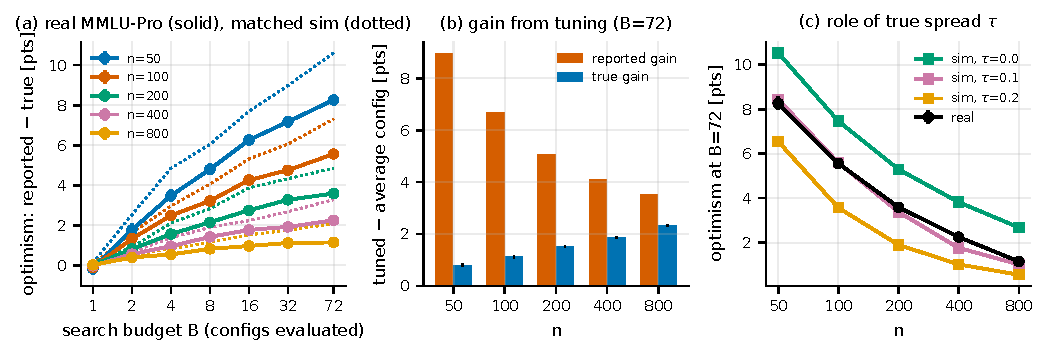
\includegraphics[width=\linewidth]{figs/fig_sweep.pdf}
\caption{\textbf{Status-quo optimism on a real LLM/benchmark.} (a) Reported minus true accuracy of the winner of random search over $B$ configurations (Qwen2.5-1.5B, MMLU-Pro; solid, $\pm1.96$ SE) and the same quantity in a synthetic world matched to the real pool's accuracy level, spread and correlation (dotted). (b) Improvement of the tuned configuration over the average configuration: reported vs.\ true. (c) Optimism at $B{=}72$ in synthetic worlds with true configuration spread $\tau$ (probit units) and on the real pool.}
\label{fig:sweep}
\end{figure}
\paragraph{Real pool.}
The 72 prompt programs are nearly interchangeable: on the \RealN\ cached questions their accuracies span \RealMin--\RealMax\% (SD \RealSD\ pts, of which about \RealNoise\ pts is evaluation noise on $|P|=\RealN$ items; the noise-corrected true spread is $\hat\tau\approx\RealTau$ pt) and the mean pairwise correlation of their per-question outcomes is \RealCorr.
Tuning by random search on $n{=}100$ questions reports an accuracy \NaiveRSNHund\ pts above the winner's true accuracy (95\% MC interval $\pm0.4$; Fig.~\ref{fig:sweep}a); at $n{=}50$ the figure is \NaiveRSNFifty, at $n{=}800$ still \NaiveRSNEightH. The reported improvement over an average configuration at $n{=}100$ is \RepGainNHund\ pts, the true one \TrueGainNHund\ pts: \FracOptNHund\% of the reported gain is optimism (Fig.~\ref{fig:sweep}b). The other search procedures behave alike (Table~\ref{tab:realopt}, App.): successive halving and the minibatch-driven surrogate search spend fewer full evaluations and over-report less (\NaiveSHNHund\ and \NaiveMIPRONHund\ pts at $n{=}100$), coordinate ascent lies in between (\NaiveCANHund).

\paragraph{Drivers.}
Equation~\eqref{eq:opt} says that optimism $=c(n)\,\mathbb{E}Z_{(B)}$ with $c=\sigma^2/\sqrt{\tau^2+\sigma^2}$, and the real pool follows it closely. \emph{Search budget:} dividing the measured optimism of random search by $\mathbb{E}Z_{(B)}$ gives a constant across $B\in\{2,\dots,72\}$ (at $n{=}100$: \CObsNHund\ pts, SD over $B$ \CObsSdNHund); even $B{=}8$ gives \NaiveRSeightNHund\ pts. \emph{Benchmark size:} $c(n)$ measured on the real pool is \CObsNFifty/\CObsNHund/\CObsNTwoH/\CObsNFourH/\CObsNEightH\ pts for $n{=}50/100/200/400/800$; the formula, fed only the pool's measured evaluation noise (config-specific part of the per-item variance, $\sigma^2\propto1/n$) and noise-corrected spread $\hat\tau$, predicts \CPredNFifty/\CPredNHund/\CPredNTwoH/\CPredNFourH/\CPredNEightH, within about 10\%. It falls between $n^{-1}$ and $n^{-1/2}$, and $n\approx800$ is needed before best-of-72 drops to about one point. \emph{True spread:} optimism is \emph{largest when configurations truly differ least} (Fig.~\ref{fig:sweep}c): $\tau{=}0$ is the worst case, and a pool whose true SD is $0.2$ probit units ($\approx7$ pts) roughly halves it at $n{=}100$. Over \TheoryCells\ simulated settings ($n$, $B$, $\tau$, between-configuration correlation) predicted and simulated optimism correlate at $r=\TheoryR$ (mean absolute error \TheoryMAE\ pts; Fig.~\ref{fig:theory}). \MatchedSentence

\begin{figure}[t]
\centering
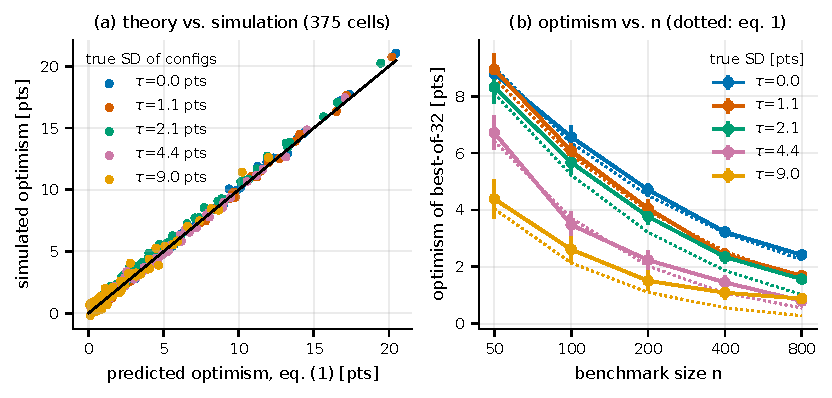
\includegraphics[width=0.78\linewidth]{figs/fig_theory.pdf}
\caption{\textbf{Closed-form optimism (eq.~\ref{eq:opt}) vs.\ simulation.} (a) 375 settings with i.i.d.\ Gaussian configuration effects (5 spreads $\times$ 3 correlations $\times$ 5 $n$ $\times$ 5 $B$). (b) Dependence on $n$ for best-of-32 ($\rho{=}0.8$); dotted = formula.}
\label{fig:theory}
\end{figure}

\subsection{Does the gap change conclusions?}
\begin{table}[t]
\centering\small
\caption{\textbf{Decisions based on reported scores.} System A = random search with $B{=}72$ on $n$ questions. It is compared on the same questions with an untuned default (a random configuration) or with a lightly tuned system (RS, $B{=}4$) by a paired one-sided $z$-test at 5\%. \emph{Claims}: share of benchmark draws declaring $A$ significantly better; \emph{false claims}: such declarations when the true gap is below 1 pt. True gap = accuracy difference of the deployed configurations over the population. 300 draws per row (real) / 150 (simulated).}
\label{tab:conc}
\begin{tabular}{lcccrr}
\toprule
 & true gap & naive gap & \multicolumn{3}{c}{claims / false claims [\%]} \\
 & [pts] & [pts] & naive & replay-boot. & hold-out \\
\midrule
real, vs.\ untuned default, $n{=}100$ & 1.1 & 6.8 & 53 / 22 & 15 / 6 & 8 / 4 \\
real, vs.\ untuned default, $n{=}400$ & 1.8 & 3.9 & 64 / 12 & 24 / 3 & 11 / 2 \\
real, vs.\ RS $B{=}4$, $n{=}100$ & 0.6 & 3.9 & 22 / 13 & 5 / 3 & 8 / 4 \\
real, vs.\ RS $B{=}4$, $n{=}400$ & 1.0 & 2.2 & 24 / 8 & 11 / 4 & 10 / 2 \\
sim, $\tau{=}0$, vs.\ untuned default, $n{=}100$ & 0.0 & 7.4 & 48 / 48 & 11 / 11 & 6 / 6 \\
sim, $\tau{=}0$, vs.\ untuned default, $n{=}400$ & 0.0 & 3.5 & 52 / 52 & 5 / 5 & 7 / 7 \\
sim, $\tau{=}0$, vs.\ RS $B{=}4$, $n{=}100$ & 0.0 & 4.0 & 9 / 9 & 3 / 3 & 9 / 9 \\
sim, $\tau{=}0$, vs.\ RS $B{=}4$, $n{=}400$ & 0.0 & 2.2 & 9 / 9 & 1 / 1 & 1 / 1 \\
sim, $\tau{=}0.1$, vs.\ untuned default, $n{=}100$ & 5.8 & 11.2 & 80 / 4 & 43 / 0 & 23 / 1 \\
sim, $\tau{=}0.1$, vs.\ untuned default, $n{=}400$ & 7.1 & 8.9 & 88 / 0 & 82 / 0 & 47 / 0 \\
sim, $\tau{=}0.1$, vs.\ RS $B{=}4$, $n{=}100$ & 2.7 & 6.6 & 38 / 5 & 23 / 2 & 15 / 2 \\
sim, $\tau{=}0.1$, vs.\ RS $B{=}4$, $n{=}400$ & 3.4 & 4.5 & 63 / 1 & 49 / 0 & 21 / 1 \\
\bottomrule
\end{tabular}

\end{table}
Table~\ref{tab:conc} shows what this does to claims. On the real pool, tuning with $B{=}72$ gives a true gain of only \TrueGapDefNHund\ pts over a random default at $n{=}100$, yet the naive paired test declares the tuned system significantly better in \ClaimNaiveDefNHund\% of benchmark draws (and in \FalseClaimNaiveDefNHund\% of draws the true gain is below one point). Against a competitor that also tuned, but with budget 4, the naive gap is \NaiveGapFourNHund\ pts against a true gap of \TrueGapFourNHund; \ClaimNaiveFourNHund\% of draws yield a significant win. At $n{=}400$ the problem persists (\ClaimNaiveDefNFourH\% claims against a \TrueGapDefNFourH-pt true gain). Hold-out reporting restores nominal behaviour (\ClaimHoldDefNHund\% claims, \FalseClaimHoldDefNHund\% false at $n{=}100$) at the price of power in a world with a real effect (simulated $\tau{=}0.1$, $n{=}100$, true gap \SynTrueGapT\ pts: \SynClaimTHold\% of draws declare a win with hold-out reporting, \SynClaimTBoot\% with the replay-bootstrap gap, \SynClaimTNaive\% naively), while with no true spread ($\tau{=}0$) the naive test declares a win in \SynClaimZNaive\% of draws against 5\% nominal (replay-bootstrap \SynClaimZBoot\%, hold-out \SynClaimZHold\%).

\subsection{Which reporting method is reliable?}
\begin{figure*}[t]
\centering
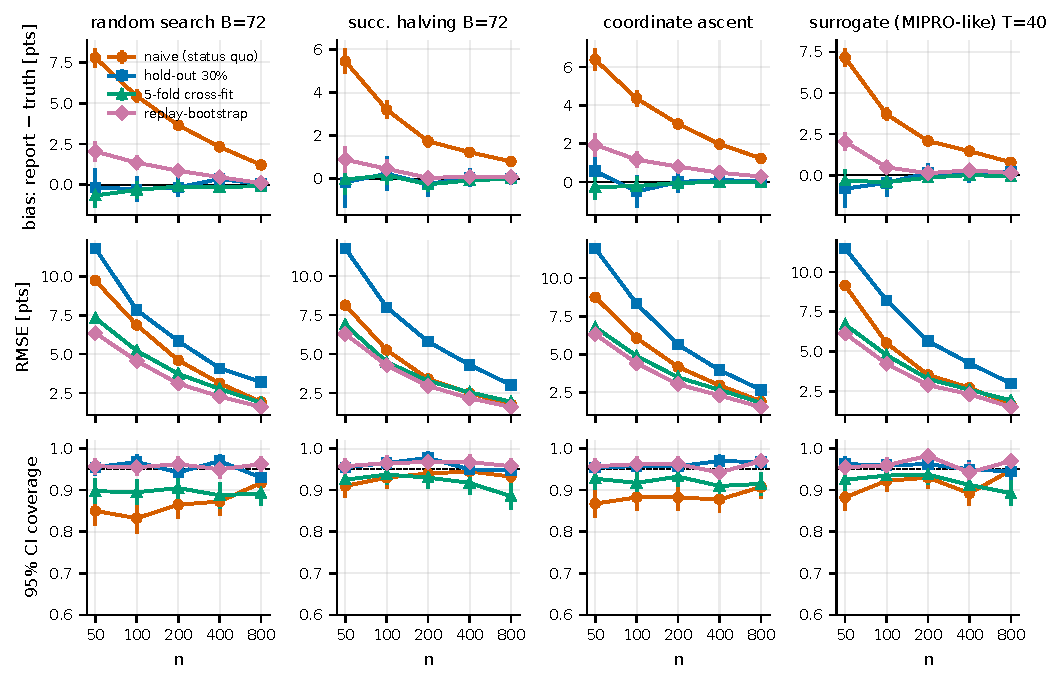
\includegraphics[width=\linewidth]{figs/fig_methods_real.pdf}
\caption{\textbf{Reporting methods on the real pool.} Bias, RMSE and coverage of nominal-95\% intervals for the accuracy of the configuration that is deployed, for four search procedures and $n$ from 50 to 800 (400 benchmark draws per cell; bars $\pm1.96$ SE). Synthetic counterparts: Fig.~\ref{fig:methods_synth} (App.).}
\label{fig:methods}
\end{figure*}
Figure~\ref{fig:methods} summarises the audit; Tables~\ref{tab:synthmeth} and~\ref{tab:extras} (App.) give numbers.
\emph{Status quo.} Biased upward everywhere; its 95\% intervals cover the winner's true accuracy only \CovNaiveRSNHund\% of the time (RS, $n{=}100$; range over cells \NaiveCovMin--\NaiveCovMax\%).
\emph{Hold-out} (30\% of $S$ reserved) is unbiased in every cell (|bias| $\le$ \HoldBiasAbsMax\ pts) and its intervals are valid (\HoldCovMin--\HoldCovMax\%), but its error is the largest: RMSE \RmseHoldRSNHund\ vs.\ \RmseNaiveRSNHund\ pts for the naive number at $n{=}100$, because $30\%$ of the data are removed from the reporting estimate \emph{and} the search sees fewer items.
\emph{Cross-fitting} (5 folds) is nearly unbiased and has lower RMSE than hold-out, but its intervals undercover (\CrossCovMin--\CrossCovMax\%) because they ignore the variability of the selection.
\emph{Replay bootstrap} (100 replays; 10 already suffice, App.~\ref{app:boot}) removes most of the bias (RS $n{=}100$: \NaiveRSNHund\ $\to$ \BootRSNHund\ pts; for SH and MIPRO-like search the residual is below 1 pt at $n\ge100$ in the real pool), has the lowest RMSE of all generic methods (\RmseBootRSNHund\ pts vs.\ \RmseNaiveRSNHund) and covers at \BootCovMin--\BootCovMax\% (nominal 95) with the same interval width as the naive one. It under-corrects when the true spread is nil and the budget large (App., Table~\ref{tab:synthmeth}): a positive residual of 1--2.5 pts.
\emph{Empirical-Bayes shrinkage} (applicable when $B$ candidates are all evaluated on $S$) is best in the real pool (RS $B{=}72$, $n{=}100$: bias \EBBias, RMSE \EBRmse\ pts, intervals \EBWidthRatio$\times$ as wide as the naive ones with \EBCov\% coverage) but it relies on a normal prior for configuration quality: in the synthetic robustness check (Table~\ref{tab:robust}) it over-shrinks a sparse set of genuinely better configurations (bias \RobSparseEBBias\ pts, coverage \RobSparseEBCov\%). The worst-case correction (subtract $\hat\sigma\,\mathbb{E}Z_{(B)}$) is as accurate on the real pool (bias \WorstBias, RMSE \WorstRmse\ pts, coverage \WorstCov\%) and degrades more gracefully (sparse pool: \RobSparseWorstBias\ pts, heavy-tailed: \RobHeavyWorstBias) because it errs on the conservative side by construction. The conditional (winner) intervals are valid in all worlds but are \CondWidthRatio$\times$ as wide as the naive ones and unbounded in a sizeable fraction of draws; simultaneous intervals are also valid but, being a statement about all candidates, do nothing about the point estimate. Ladder reduces the bias only partially (RS: \LadderBias\ pts, coverage \LadderCov\%) and Thresholdout with a half-split of $S$ and noisy answers is \emph{worse} than doing nothing at these budgets (\ThoBias\ pts), as its guarantees need far more data per query.

\subsection{Further diagnostics}
\paragraph{Demonstrations drawn from the benchmark leak their own answers.}
Optimisers such as DSPy's \texttt{BootstrapFewShot} take demonstrations from the tuning set, so the tuned prompt contains the answer to some of the items on which it is then scored. With the same prompt format as above, accuracy on the three items shown as demonstrations is \LeakIn\% versus \LeakOut\% on other items (\LeakSets\ random demonstration sets), i.e.\ about $+45$ pts per leaked item: $3$-shot bootstrapped demonstrations add roughly $1.4$ pts to a report at $n{=}100$ on top of the selection effect (arithmetic from these two numbers; not an end-to-end DSPy run).
\paragraph{A label-permutation negative control.} Re-scoring the cached predictions against permuted gold labels (all configurations then truly at chance) and re-running the search measures what the procedure can fabricate from noise alone. Its optimism is a fraction \PermRatioMin--\PermRatioMax\ (median \PermRatioMed) of the optimism measured with real labels (App.), a cheap audit of how much of a reported gain a search of that size and benchmark size could produce spuriously; it is not an unbiased estimator because the noise level depends on accuracy.
\paragraph{How much data should reporting get?}
For random search with $B{=}72$ and $n{=}100$ on the real pool, reserving 10\%/30\%/50\% of the benchmark for reporting gives hold-out RMSE \FrRmseTenNHund/\FrRmseThirtyNHund/\FrRmseFiftyNHund\ pts (naive: \FrRmseNaiveNHund; replay bootstrap: \RmseBootRSNHund), while the true accuracy of the configuration deployed falls by only \FrLossTenNHund/\FrLossThirtyNHund/\FrLossFiftyNHund\ pts, because searching with fewer items hardly matters when the candidates are nearly equivalent. In a simulated world with real spread ($\tau{=}0.1$) the same loss is \FrSynLossTenNHund/\FrSynLossThirtyNHund/\FrSynLossFiftyNHund\ pts. The price of an unbiased report is thus mainly precision of the report, not the quality of the system; in small benchmarks the replay bootstrap offers a better error trade-off.
\paragraph{A pool with real signal (Real-II).}
To check that the picture is not specific to a pool of near-equivalent prompts, we built a second real pool from four small models (Qwen2.5-1.5B, Qwen2-1.5B, Qwen3-1.7B, Qwen3-0.6B) $\times$ 8 prompt variants (zero-/3-shot, 2 instructions, 2 cues), i.e.\ $K{=}\RTwoK$ configurations scored on \RTwoN\ questions (smaller because of compute; App.~\ref{app:real2}). Here the pool's accuracies span \RTwoMin--\RTwoMax\% (SD \RTwoSD\ pts), driven mostly by model identity. Random search over all 32 on $n{=}100$ questions still over-reports by \RTwoNaiveNHund\ pts, presumably because the final choice is among near-equivalent prompts of the best model(s); replay bootstrap and hold-out give \RTwoBootNHund\ and \RTwoHoldNHund\ (coverage \RTwoCovBootNHund\% and \RTwoCovHoldNHund\% vs.\ \RTwoCovNaiveNHund\% naive). Larger spread across models does not make the reported number trustworthy when the final choice is made among close competitors.
